\documentclass[10pt]{article}
\usepackage[margin=0.7in]{geometry}
\usepackage[T1]{fontenc}
\usepackage{graphicx,hyperref}
\begin{document}
\section*{Independent same-root composition review}
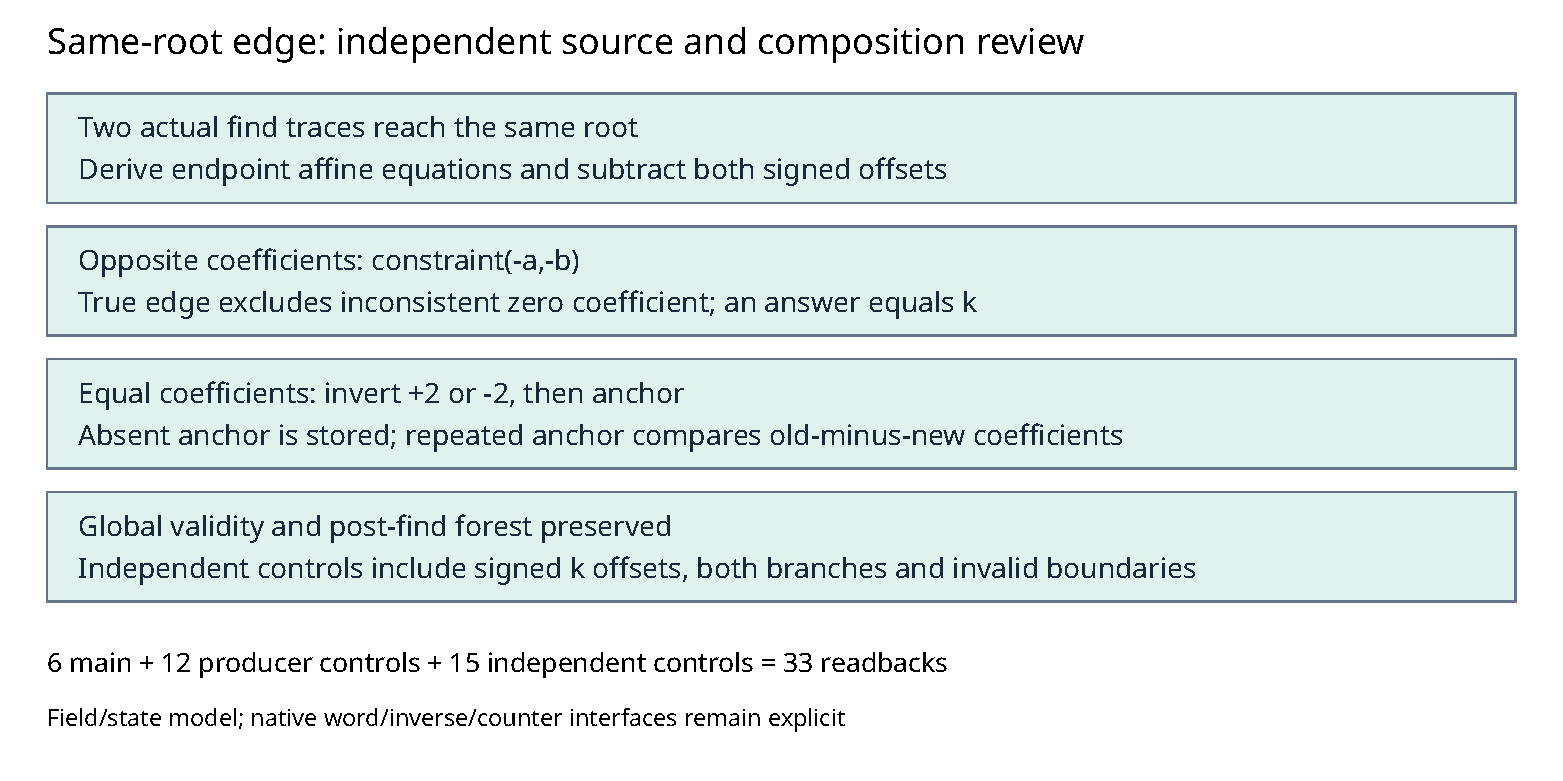
\includegraphics[width=\linewidth]{flow.pdf}

Six producer declarations, twelve producer controls and fifteen independent controls passed fresh native Lean replay: thirty-three exact named readbacks. An independent Rust checker validates module order, native exits, source bytes, snapshot hashes and allowed axioms. A fresh false equality returned native and runner exit1.

\paragraph{Source fidelity.}
Native constraint returns $-a/b$ for nonzero $b$ and otherwise asserts $a=0$. The model explicitly represents inconsistency. Anchor either compares old-minus-new coefficients or stores only the absent selected entry. The same-root branch follows two actual finds, reduces both signed offsets, and uses either constraint$(-a,-b)$ or the inverse of $+2$/$-2$.

\paragraph{Composition.}
The theorem derives endpoint equations from actual recursive Run traces and initial Forest/Valid. It does not assume the desired root value, final invariant, absence of assertion, or answer. The shared returned root matches the native branch condition. Global anchor and vertex equations survive the update; the post-find graph is unchanged.

\newpage
\section*{Controls, custody and scope}
\paragraph{Independent fixture.}
A four-node signed graph uses nonzero target coefficients on both descendants: $+k$ and $-k$. Two nontrivial finds reach root1. Opposite coefficients return scalar2. Equal negative coefficients use the $-2$ denominator and store anchor$(3,0)$. The reserved node0 anchor is preserved. Additional controls cover repeated consistent anchors, repeated scalar recovery, contradictory anchors, characteristic2, nonsigns and assertion exclusion.

\paragraph{Custody and independence.}
Review follows published commit b4684a67ca626d338099525aefae817a3d276e78. Nine mathematical source modules and Rust runner source match published bytes; all1146 producer manifest entries matched. Native source was read before theorem inspection; the local written plan followed initial inspection. The prospective joint is the published coordinator plan. Prior imported GraphAlgebra authorship and source familiarity are disclosed; no fully blind claim is made.

\paragraph{Boundaries.}
Field coefficients, nonzero2, true incoming edge, initial invariant and signed coefficients are explicit. Ring::new asserts prime order greater than2, but word decoding and inversion are not composed here. Native signed dispatch, counter and arithmetic overflow, arrays and compiled execution remain separate interfaces. Inconsistency represents the native assertion; invalid inputs are not claimed to return normally.

\paragraph{Workflow and failures.}
The published Rust runner was rebuilt offline. Nine producer modules and eleven reviewer modules passed fresh runs. An initial shell command guessed a nonexistent executable name and exited127 before replay; corrected invocation used the declared package name. No reviewer Lean proof failed. Producer failures remain retained. No Python verifier, scientific execution, cloud change or repository edit occurred.

\paragraph{Evidence.}
See REPORT.md, status.json, attestation.json, acceptance.json, producer-replay-acceptance.json, and the replay1/reviewer1/known-false directories. Result: machine checks passed and source fidelity validated at the stated scope. Official research decisions remain with the Coordinator.
\end{document}
